\chapter{The Eagle Squad}
\label{chap:squad}

You will fly missions for the Eagle Squad, which
is known for a good equipment and the best pilots.
Just look at the fighter and pilot overviews.


\section{The Fighters}
\label{sec:fighters}

\begin{center}
\begin{tabular}{p{3cm}p{3cm}p{3cm}p{3cm}}
GL-16 Falcon: &
Crow: &
GL-22: Hawk &
Swallow:\\
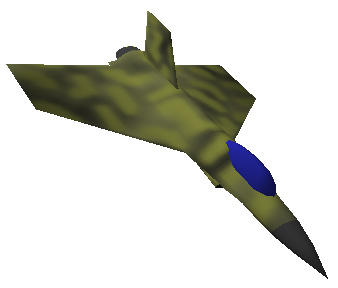
\includegraphics[width=4cm]{falcon.jpg} &
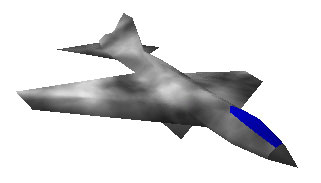
\includegraphics[width=4cm]{crow.jpg} &
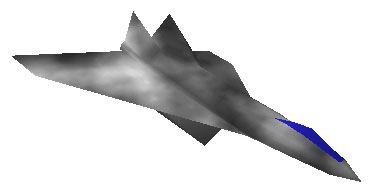
\includegraphics[width=4cm]{hawk.jpg} &
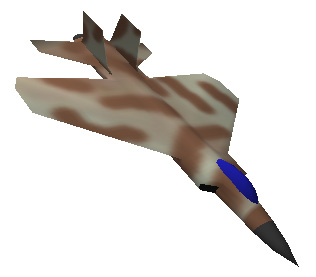
\includegraphics[width=4cm]{swallow.jpg}\\
\end{tabular}
\end{center}

The GL-16 is the Eagle Squad's fighter used to get rid of bombers like the Swallow,
whereas the GL-22 can take more missiles at the cost of manoeverability.
At the beginning of each mission, you can decide which fighter to take, but be careful:
only the heavy bombers have enough firepower to destroy static buildings.


\section{The Weapons}
\label{sec:weapons}

\begin{center}
\begin{tabular}{p{3cm}p{3cm}p{3cm}p{3cm}}
FF (friend-foe): &
IR (infra-red): &
AGM (air-gr.): &
DF (dumb fire):\\
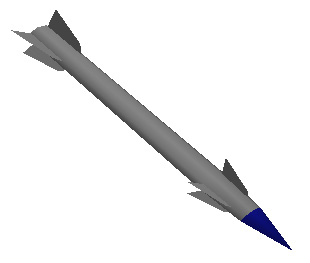
\includegraphics[width=3cm]{missile_ff.jpg} &
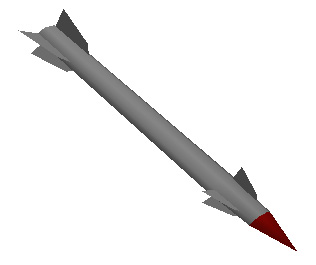
\includegraphics[width=3cm]{missile_ir.jpg} &
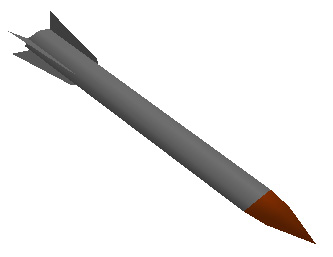
\includegraphics[width=3cm]{missile_agm.jpg} &
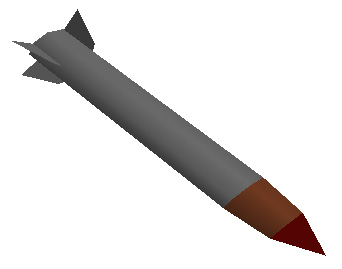
\includegraphics[width=3cm]{missile_df.jpg}\\
\end{tabular}
\end{center}

Use FF missiles early when approaching the enemy.
They will search their target using a radar system,
however a chaff cloud may fool them.

IR missiles can only track the enemy by heat and must
therefore be fired at the enemy's back.
Flares consisting of burning magnesium can be used as a countermeasure.

AGMs are radar controlled missiles used to
take out medium ground targets like tanks.

DF missiles will only fly straight ahead like cannon shots,
but can cause an enormous amount of damage,
so they are used to take out huge ground targets like buildings.
